\PassOptionsToPackage{unicode=true}{hyperref} % options for packages loaded elsewhere
\PassOptionsToPackage{hyphens}{url}
%
\documentclass[ignorenonframetext,]{beamer}
\usepackage{pgfpages}
\setbeamertemplate{caption}[numbered]
\setbeamertemplate{caption label separator}{: }
\setbeamercolor{caption name}{fg=normal text.fg}
\beamertemplatenavigationsymbolsempty
\usepackage{lmodern}
\usepackage{amssymb,amsmath}
\usepackage{ifxetex,ifluatex}
\usepackage{fixltx2e} % provides \textsubscript
\ifnum 0\ifxetex 1\fi\ifluatex 1\fi=0 % if pdftex
  \usepackage[T1]{fontenc}
  \usepackage[utf8]{inputenc}
  \usepackage{textcomp} % provides euro and other symbols
\else % if luatex or xelatex
  \usepackage{unicode-math}
  \defaultfontfeatures{Ligatures=TeX,Scale=MatchLowercase}
\fi
% use upquote if available, for straight quotes in verbatim environments
\IfFileExists{upquote.sty}{\usepackage{upquote}}{}
% use microtype if available
\IfFileExists{microtype.sty}{%
\usepackage[]{microtype}
\UseMicrotypeSet[protrusion]{basicmath} % disable protrusion for tt fonts
}{}
\IfFileExists{parskip.sty}{%
\usepackage{parskip}
}{% else
\setlength{\parindent}{0pt}
\setlength{\parskip}{6pt plus 2pt minus 1pt}
}
\usepackage{hyperref}
\hypersetup{
            pdftitle={Reproducible Workflow: Software},
            pdfborder={0 0 0},
            breaklinks=true}
\urlstyle{same}  % don't use monospace font for urls
\newif\ifbibliography
\usepackage{color}
\usepackage{fancyvrb}
\newcommand{\VerbBar}{|}
\newcommand{\VERB}{\Verb[commandchars=\\\{\}]}
\DefineVerbatimEnvironment{Highlighting}{Verbatim}{commandchars=\\\{\}}
% Add ',fontsize=\small' for more characters per line
\usepackage{framed}
\definecolor{shadecolor}{RGB}{248,248,248}
\newenvironment{Shaded}{\begin{snugshade}}{\end{snugshade}}
\newcommand{\AlertTok}[1]{\textcolor[rgb]{0.94,0.16,0.16}{#1}}
\newcommand{\AnnotationTok}[1]{\textcolor[rgb]{0.56,0.35,0.01}{\textbf{\textit{#1}}}}
\newcommand{\AttributeTok}[1]{\textcolor[rgb]{0.77,0.63,0.00}{#1}}
\newcommand{\BaseNTok}[1]{\textcolor[rgb]{0.00,0.00,0.81}{#1}}
\newcommand{\BuiltInTok}[1]{#1}
\newcommand{\CharTok}[1]{\textcolor[rgb]{0.31,0.60,0.02}{#1}}
\newcommand{\CommentTok}[1]{\textcolor[rgb]{0.56,0.35,0.01}{\textit{#1}}}
\newcommand{\CommentVarTok}[1]{\textcolor[rgb]{0.56,0.35,0.01}{\textbf{\textit{#1}}}}
\newcommand{\ConstantTok}[1]{\textcolor[rgb]{0.00,0.00,0.00}{#1}}
\newcommand{\ControlFlowTok}[1]{\textcolor[rgb]{0.13,0.29,0.53}{\textbf{#1}}}
\newcommand{\DataTypeTok}[1]{\textcolor[rgb]{0.13,0.29,0.53}{#1}}
\newcommand{\DecValTok}[1]{\textcolor[rgb]{0.00,0.00,0.81}{#1}}
\newcommand{\DocumentationTok}[1]{\textcolor[rgb]{0.56,0.35,0.01}{\textbf{\textit{#1}}}}
\newcommand{\ErrorTok}[1]{\textcolor[rgb]{0.64,0.00,0.00}{\textbf{#1}}}
\newcommand{\ExtensionTok}[1]{#1}
\newcommand{\FloatTok}[1]{\textcolor[rgb]{0.00,0.00,0.81}{#1}}
\newcommand{\FunctionTok}[1]{\textcolor[rgb]{0.00,0.00,0.00}{#1}}
\newcommand{\ImportTok}[1]{#1}
\newcommand{\InformationTok}[1]{\textcolor[rgb]{0.56,0.35,0.01}{\textbf{\textit{#1}}}}
\newcommand{\KeywordTok}[1]{\textcolor[rgb]{0.13,0.29,0.53}{\textbf{#1}}}
\newcommand{\NormalTok}[1]{#1}
\newcommand{\OperatorTok}[1]{\textcolor[rgb]{0.81,0.36,0.00}{\textbf{#1}}}
\newcommand{\OtherTok}[1]{\textcolor[rgb]{0.56,0.35,0.01}{#1}}
\newcommand{\PreprocessorTok}[1]{\textcolor[rgb]{0.56,0.35,0.01}{\textit{#1}}}
\newcommand{\RegionMarkerTok}[1]{#1}
\newcommand{\SpecialCharTok}[1]{\textcolor[rgb]{0.00,0.00,0.00}{#1}}
\newcommand{\SpecialStringTok}[1]{\textcolor[rgb]{0.31,0.60,0.02}{#1}}
\newcommand{\StringTok}[1]{\textcolor[rgb]{0.31,0.60,0.02}{#1}}
\newcommand{\VariableTok}[1]{\textcolor[rgb]{0.00,0.00,0.00}{#1}}
\newcommand{\VerbatimStringTok}[1]{\textcolor[rgb]{0.31,0.60,0.02}{#1}}
\newcommand{\WarningTok}[1]{\textcolor[rgb]{0.56,0.35,0.01}{\textbf{\textit{#1}}}}
\usepackage{graphicx,grffile}
\makeatletter
\def\maxwidth{\ifdim\Gin@nat@width>\linewidth\linewidth\else\Gin@nat@width\fi}
\def\maxheight{\ifdim\Gin@nat@height>\textheight\textheight\else\Gin@nat@height\fi}
\makeatother
% Scale images if necessary, so that they will not overflow the page
% margins by default, and it is still possible to overwrite the defaults
% using explicit options in \includegraphics[width, height, ...]{}
\setkeys{Gin}{width=\maxwidth,height=\maxheight,keepaspectratio}
% Prevent slide breaks in the middle of a paragraph:
\widowpenalties 1 10000
\raggedbottom
\setbeamertemplate{part page}{
\centering
\begin{beamercolorbox}[sep=16pt,center]{part title}
  \usebeamerfont{part title}\insertpart\par
\end{beamercolorbox}
}
\setbeamertemplate{section page}{
\centering
\begin{beamercolorbox}[sep=12pt,center]{part title}
  \usebeamerfont{section title}\insertsection\par
\end{beamercolorbox}
}
\setbeamertemplate{subsection page}{
\centering
\begin{beamercolorbox}[sep=8pt,center]{part title}
  \usebeamerfont{subsection title}\insertsubsection\par
\end{beamercolorbox}
}
\AtBeginPart{
  \frame{\partpage}
}
\AtBeginSection{
  \ifbibliography
  \else
    \frame{\sectionpage}
  \fi
}
\AtBeginSubsection{
  \frame{\subsectionpage}
}
\setlength{\emergencystretch}{3em}  % prevent overfull lines
\providecommand{\tightlist}{%
  \setlength{\itemsep}{0pt}\setlength{\parskip}{0pt}}
\setcounter{secnumdepth}{0}

% set default figure placement to htbp
\makeatletter
\def\fps@figure{htbp}
\makeatother


\title{Reproducible Workflow: Software}
\providecommand{\subtitle}[1]{}
\subtitle{Quick Overviews of Version Control (Github) and Dynamic Documents
(RMarkdown)}
\author{Fernando Hoces de la Guardia\\
BITSS\\
-\\
Slides at \url{https://goo.gl/aBQ3LR}}
\date{Inter-American Development Bank Workshop, March 2018}

\begin{document}
\frame{\titlepage}

\begin{frame}
\tableofcontents[hideallsubsections]
\end{frame}
\begin{frame}{The Claerbout Principle}
\protect\hypertarget{the-claerbout-principle}{}

\begin{quote}
An article about computational science in a scientific publication is
not the scholarship itself, it is merely advertising of the scholarship.
The actual scholarship is the complete software development environment
and the complete set of instructions which generated the figures.
\end{quote}

\href{https://statweb.stanford.edu/~wavelab/Wavelab_850/wavelab.pdf}{Buckheit
\& Donoho, 1995}

\end{frame}

\begin{frame}{Organizing Principles}
\protect\hypertarget{organizing-principles}{}

1 - Use code (scripts), don't work by hand (Excel/spreadsheet, GUIs). 2
- Consider not saving statistical output, and just saving the code and
raw data that generates it. 3 - Reproducibility--on your own machine
across multiple runs, across machines, across researchers.

\end{frame}

\begin{frame}{File Management \& Coding Suggestions}
\protect\hypertarget{file-management-coding-suggestions}{}

Begin with a logical file structure
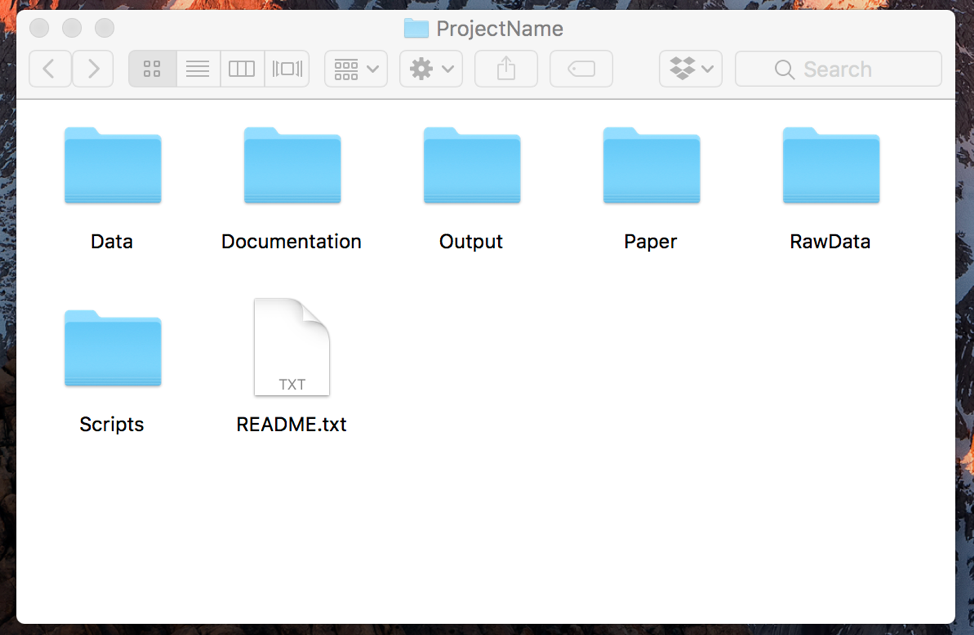
\includegraphics[height=2.25in]{../Images/files.png}

\end{frame}

\begin{frame}{General Coding Suggestions I (Christensen, Miguel \&
Freese, 2018)}
\protect\hypertarget{general-coding-suggestions-i-christensen-miguel-freese-2018}{}

\begin{itemize}
\item
  Make sure script files are self-contained: don't write code that only
  works if you run a group of other files previously in a specific order
  and then leave things hanging precariously.
\item
  Include tests in your code.\\
  This can alert you if output changes.
\item
  You can never comment your code too much. Truly explain rather than
  transliterating: \texttt{x=1} as ``initialize the population count to
  1'' or ``set x equal to 1.''
\item
  Indent your code.
\end{itemize}

\end{frame}

\begin{frame}{General Coding Suggestions II}
\protect\hypertarget{general-coding-suggestions-ii}{}

\begin{itemize}
\tightlist
\item
  Once posted, any changes at all require a new file name. Better: use
  version control.\\
\item
  Separate your data cleaning and analysis files. Don't make any new
  variables that need saving (or will be used by multiple analysis
  files) in an analysis file. It is far better to only create a variable
  once so you know that it is identical when used in different analysis
  files.
\end{itemize}

\end{frame}

\begin{frame}[fragile]{General Coding Suggestions III}
\protect\hypertarget{general-coding-suggestions-iii}{}

\begin{itemize}
\tightlist
\item
  Name variables informatively: pick a side for indicator variables
  \texttt{dead"\ (or}living'') instead of ``status". (gender, race,
  etc.)
\item
  Don't leave clutter around-delete temporary or unnecessary
  intermediate objects.

  \item

  You can use a prefix such as \texttt{x\_} or \texttt{temp\_} so you
  know which files or variables can easily be deleted later. Stata also
  has the \texttt{tempfile} and \texttt{tempvar} functionality.\\
\item
  Every variable should have a label. (If allowed for by the program.)
\item
  Use relative directory paths (such as \texttt{./Data} not
  \texttt{C:/Users/garret/Documents/Project/Data})
\end{itemize}

\end{frame}

\begin{frame}{Managing expectations}
\protect\hypertarget{managing-expectations}{}

\begin{figure}
\centering
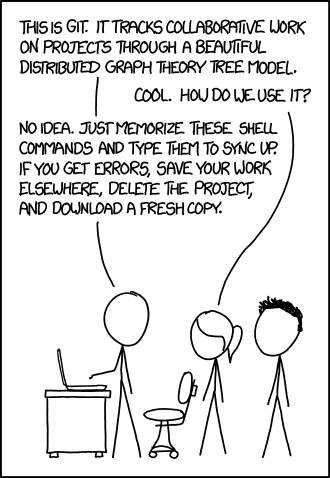
\includegraphics{https://imgs.xkcd.com/comics/git.png}
\caption{Git xkcd comic}
\end{figure}

\end{frame}

\begin{frame}[fragile]{The Primary Goal of Version Control (for us)}
\protect\hypertarget{the-primary-goal-of-version-control-for-us}{}

\textbf{The Goal:} keep track of any potentially meaningfull
modification to your code (Git is also great for collaboration and
exploring the work of others).

\#\#Strategy 1:\\
1 - Agree on a naming convention with you co-authors (eg:
YYYYMMDDfilename\_INITALS).\\
2 - Begin working from the last saved version (eg:
\texttt{20180325demo\_FH.do}).\\
3 - At the end of the day, save on a new version (eg:
\texttt{20180327demo\_FH.do}).

\textbf{Pros:} Easy adoption.

\textbf{Cons:} Error prone, hard to document, lots of files for each
document.

\#\#Strategy 2:\\
1 - Name your file \texttt{filename} (ideally \texttt{01\_filename})\\
2 - Take a snapshot of your work every time you complete relevant change
(day, hour or minutes).\\
3 - Update your entire working folder to the cloud.

\textbf{Pros:} Error proof, seemless documentation, one file per
document, track differences across all versions, meant to work with the
cloud.

\textbf{Cons:} Harder adoption.

\end{frame}

\begin{frame}{Tips to ease the adoption: concepts.}
\protect\hypertarget{tips-to-ease-the-adoption-concepts.}{}

\begin{itemize}
\tightlist
\item
  \textbf{Git} is the software that does all the magic. \textbf{Github}
  is an implementation of Git that is easier to use, provides free
  (public) cloud service, and tools for collaboration.
\item
  A repository (\textbf{repo}) is a master folder that contains all your
  work.
\item
  Whenever you take a snapshot of your \emph{saved} work, you
  \textbf{commit}
\item
  When you make changes to your files in your computer, you are working
  \textbf{locally}, whenever you make changes to the files in the cloud
  you are working \textbf{remotelly}.
\item
  Whenever you want to update your \emph{remote} \emph{repo}, you
  \textbf{push}. If you want to update you \emph{local} \emph{repo}, you
  \textbf{pull}.
\item
  When you copy a repo from another person into your online github
  account, you \textbf{fork} it.
\item
  When you start a repo from github.com (just created or forked), and
  want to download it for the first time to your local computer, you
  \textbf{clone} it.
\end{itemize}

\end{frame}

\begin{frame}[fragile]{Tips to ease the adoption: 4 min tutorial.}
\protect\hypertarget{tips-to-ease-the-adoption-4-min-tutorial.}{}

1- Create \url{github.com} account and sign in. {[}1 min{]}\\
2- Search \texttt{BITSS\ AIR} 3- Fork it.{[}1min{]}\\
4- (You have left the BITSS account, and are now in your account)\\
5- Click on \texttt{README.md}, then click on the pencil icon {[}1min{]}

\includegraphics{edit.png}

\end{frame}

\begin{frame}[fragile]{Tips to ease the adoption: 4 min tutorial.}
\protect\hypertarget{tips-to-ease-the-adoption-4-min-tutorial.-1}{}

6- Modify the title (\texttt{\#\ AIR\ Reproducibility\ Training}) and
click \texttt{Commit\ changes}\\
7- Go back to the root folder of the repo (\texttt{AIRMay2018}), and
click \texttt{Clone\ or\ download}. And download as a zip.

If you had \href{https://desktop.github.com/}{Github Desktop} (an app
from the Github company) installed, you could clone the repo and play
more.

But I just wanted to give you a quick intro to:\\
- Find code of interest, fork it, edit it, make your first commit, and
download.

\end{frame}

\begin{frame}{Want to learn more:}
\protect\hypertarget{want-to-learn-more}{}

\begin{itemize}
\item
  \href{https://www.youtube.com/watch?v=eWxxfttcMts}{Great 20 min intro
  to Git by Alice Bartlett}
\item
  \href{https://www.rstudio.com/resources/videos/happy-git-and-gihub-for-the-user-tutorial/}{Great
  2hr tutorial to Github by Jenny Bryan (git ninja)}
\item
  \href{http://web.stanford.edu/~gentzkow/research/CodeAndData.pdf}{Documentation
  from Matthew Gentzkow Jesse Shapiro}
\item
  Come to 3-Day trainning (RT2) in Seattle
  (\href{https://www.bitss.org/events/research-transparency-and-reproducibility-training-rt2-amsterdam/}{Amsterdam
  next week}, \href{https://github.com/BITSS/RT2Berkeley2017}{repo from
  last year})!
\end{itemize}

\end{frame}

\hypertarget{dynamic-documents}{%
\section{Dynamic Documents}\label{dynamic-documents}}

\begin{frame}[fragile]{Dynamic Documents For Computational
Reproducibility}
\protect\hypertarget{dynamic-documents-for-computational-reproducibility}{}

\begin{itemize}
\tightlist
\item
  Based on principles of \emph{literate programming} aims at combining
  code and paper in one single document
\item
  Best framework to achieve the holy grail of \textbf{one-click
  reproducible workflow}
\item
  Best two current implementations: \texttt{RMarkdown\ (R)} \&
  \texttt{Jupyter\ (Python)}. \texttt{Stata} is catching up (dyndocs
  release \href{https://www.stata.com/new-in-stata/markdown/}{here} and
  reviews
  \href{http://data.princeton.edu/stata/markdown/markstat.htm}{here} and
  \href{https://www.bitss.org/2017/09/05/review-of-statas-dyndoc/}{here})
\end{itemize}

\end{frame}

\begin{frame}{Currently code and narrative components live in separate
universes}
\protect\hypertarget{currently-code-and-narrative-components-live-in-separate-universes}{}

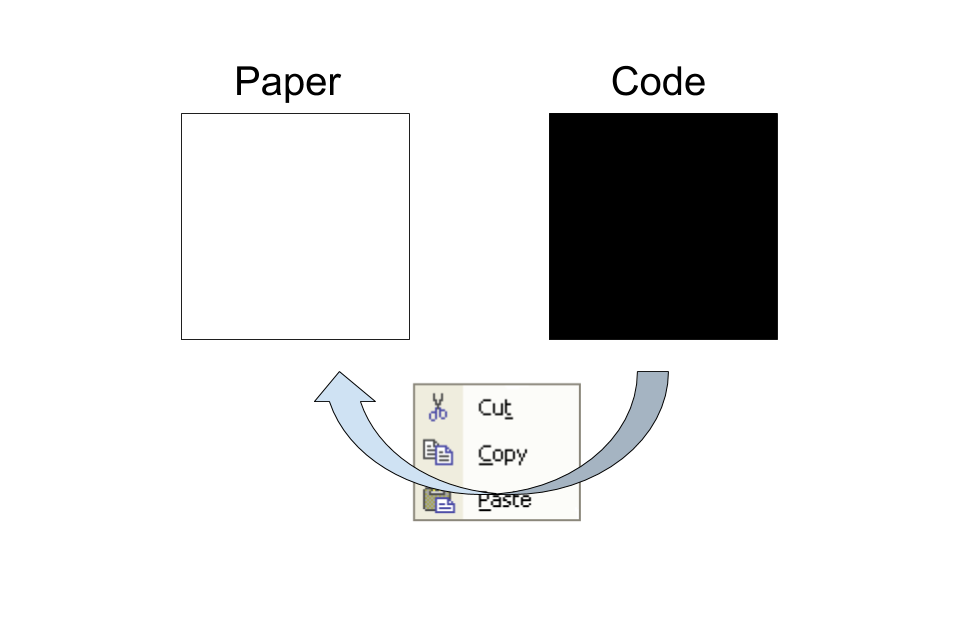
\includegraphics{./Two universes.png}

\end{frame}

\begin{frame}{Dynamic Documents: integrate the two universes!}
\protect\hypertarget{dynamic-documents-integrate-the-two-universes}{}


\includegraphics{./One universe.png}

\end{frame}

\begin{frame}[fragile]{Dynamic Documents: A Recipe}
\protect\hypertarget{dynamic-documents-a-recipe}{}

\begin{itemize}
\tightlist
\item
  1 simple language that can combine text and code: \texttt{Markdown}
\item
  1 statistical package to do the analysis (\texttt{R}, \texttt{Python},
  \texttt{3S\textquotesingle{}s?})
\item
  1 machinery to combine analysis and text to create a single output:
  \texttt{Pandoc}
\item
  {[}Optional-but-not-really{]} 1 program to bring all the elements
  together: RStudio/RMarkdown, Jupyter
\end{itemize}

\end{frame}

\begin{frame}[fragile]{Basic Structure: Code Chunks and Inline}
\protect\hypertarget{basic-structure-code-chunks-and-inline}{}

\begin{Shaded}
\begin{Highlighting}[]
\OperatorTok{---}
\NormalTok{header}
\OperatorTok{---}
\end{Highlighting}
\end{Shaded}

Body of text.

To begin a piece of code (``code chunk''). Enclose them in the following
expression (Ctrl/Cmd + shift/optn + i)

\begin{verbatim}
```{r, eval=TRUE}
here goes the code
```
\end{verbatim}

To write inline use only one Backtick to open followed by an ``r''" and
one to close \texttt{\textasciigrave{}r\ 1+1\textasciigrave{}} in the
output.

\end{frame}

\begin{frame}{P-hacking with the little experiment}
\protect\hypertarget{p-hacking-with-the-little-experiment}{}

\begin{itemize}
\tightlist
\item
  OLS
\item
  3 outputs
\item
  2 Treatment vars\\
\item
  7 Possible covariates (6 + none)\\
\item
  Total of 42 plausible models
\end{itemize}

\end{frame}

\begin{frame}{P-Hacking in Action (Specification Curve)}
\protect\hypertarget{p-hacking-in-action-specification-curve}{}

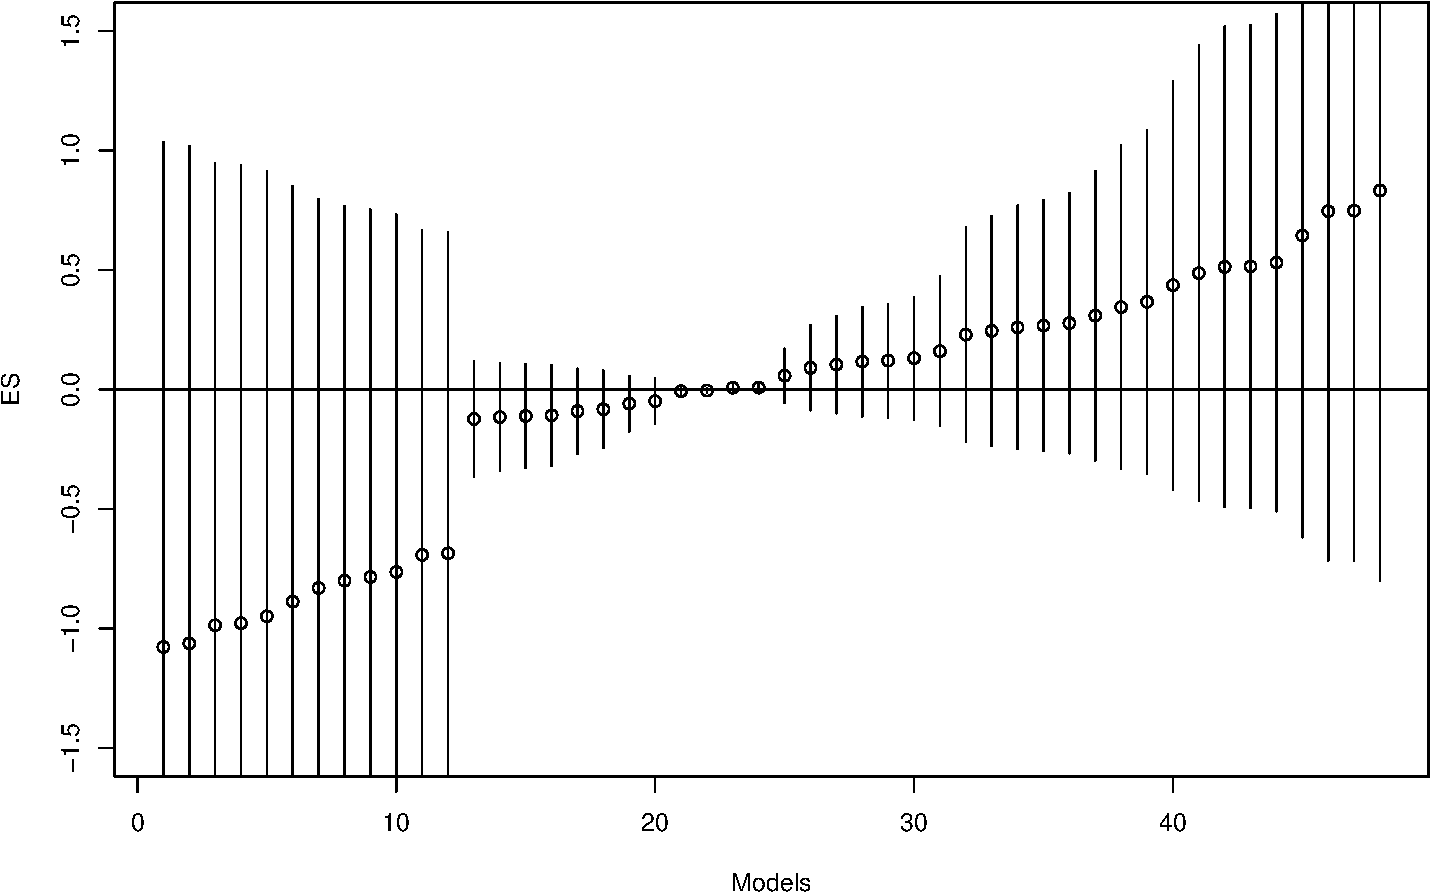
\includegraphics{rep_workflow_slides_files/figure-beamer/spec curve-1.pdf}

\end{frame}

\begin{frame}{Back-up Demo: The Birthday Problem!}
\protect\hypertarget{back-up-demo-the-birthday-problem}{}

As an illustration lets write a report using the participants in this
workshop to illustrate the famous
\href{https://en.wikipedia.org/wiki/Birthday_problem}{birthday problem}.

\begin{quote}
What is the probability that at least two people this room share the
same birthday?
\end{quote}

\begin{quote}
Is it something like \(\frac{1}{365} \times N =\) 0.058?
\end{quote}

\end{frame}

\begin{frame}[fragile]{Create a new RMarkdown File}
\protect\hypertarget{create-a-new-rmarkdown-file}{}

1 - In RStudio:
\texttt{File-\textgreater{}\ New\ File\ -\textgreater{}\ RMarkdown...}\\
2 - Name it, and save it.\\
3 - Review/edit the header, and delete all the default body of text
except for one code chunk.\\
4 - Define a seed (\texttt{set.seed(1234)} and number of people in the
room (\texttt{n.pers\ =\ ?})

\end{frame}

\begin{frame}{The birthday problem: the math}
\protect\hypertarget{the-birthday-problem-the-math}{}

Actually the math says otherwise: \begin{align} 
 1 - \bar p(n) &= 1 \times \left(1-\frac{1}{365}\right) \times \left(1-\frac{2}{365}\right) \times \cdots \times \left(1-\frac{n-1}{365}\right) \nonumber  \\  &= \frac{ 365 \times 364 \times \cdots \times (365-n+1) }{ 365^n } \nonumber \\ &= \frac{ 365! }{ 365^n (365-n)!} = \frac{n!\cdot\binom{365}{n}}{365^n}\\
p(n= 21) &= 0.444  \nonumber
\end{align}

\end{frame}

\begin{frame}[fragile]{Code for the math (\url{https://goo.gl/ZFQvba})}
\protect\hypertarget{code-for-the-math-httpsgoo.glzfqvba}{}

Don't look at this: just copy and paste into your report

\begin{Shaded}
\begin{Highlighting}[]
\NormalTok{\textbackslash{}begin\{align\} }
 \DecValTok{1} \OperatorTok{-}\StringTok{ }\NormalTok{\textbackslash{}bar }\KeywordTok{p}\NormalTok{(n) }\OperatorTok{&}\ErrorTok{=}\StringTok{ }\DecValTok{1}\NormalTok{ \textbackslash{}times \textbackslash{}}\KeywordTok{left}\NormalTok{(}\DecValTok{1}\OperatorTok{-}\NormalTok{\textbackslash{}frac\{}\DecValTok{1}\NormalTok{\}\{}\DecValTok{365}\NormalTok{\}\textbackslash{}right) }
\NormalTok{ \textbackslash{}times \textbackslash{}}\KeywordTok{left}\NormalTok{(}\DecValTok{1}\OperatorTok{-}\NormalTok{\textbackslash{}frac\{}\DecValTok{2}\NormalTok{\}\{}\DecValTok{365}\NormalTok{\}\textbackslash{}right) \textbackslash{}times \textbackslash{}cdots \textbackslash{}times }
\NormalTok{ \textbackslash{}}\KeywordTok{left}\NormalTok{(}\DecValTok{1}\OperatorTok{-}\NormalTok{\textbackslash{}frac\{n}\DecValTok{-1}\NormalTok{\}\{}\DecValTok{365}\NormalTok{\}\textbackslash{}right) \textbackslash{}nonumber  \textbackslash{}\textbackslash{}  }
 \OperatorTok{&}\ErrorTok{=}\StringTok{ }\NormalTok{\textbackslash{}frac\{ }\DecValTok{365}\NormalTok{ \textbackslash{}times }\DecValTok{364}\NormalTok{ \textbackslash{}times \textbackslash{}cdots \textbackslash{}times }
\NormalTok{   (}\DecValTok{365}\OperatorTok{-}\NormalTok{n}\OperatorTok{+}\DecValTok{1}\NormalTok{) \}\{ }\DecValTok{365}\OperatorTok{^}\NormalTok{n \} \textbackslash{}nonumber \textbackslash{}\textbackslash{} }
 \OperatorTok{&}\ErrorTok{=}\StringTok{ }\NormalTok{\textbackslash{}frac\{ }\DecValTok{365}\OperatorTok{!}\StringTok{ }\NormalTok{\}\{ }\DecValTok{365}\OperatorTok{^}\KeywordTok{n}\NormalTok{ (}\DecValTok{365}\OperatorTok{-}\NormalTok{n)}\OperatorTok{!}\NormalTok{\} =}\StringTok{ }
\StringTok{   }\NormalTok{\textbackslash{}frac\{n}\OperatorTok{!}\NormalTok{\textbackslash{}cdot\textbackslash{}binom\{}\DecValTok{365}\NormalTok{\}\{n\}\}\{}\DecValTok{365}\OperatorTok{^}\NormalTok{n\}\textbackslash{}\textbackslash{}}
\KeywordTok{p}\NormalTok{(}\DataTypeTok{n=} \StringTok{`}\DataTypeTok{r n.pers}\StringTok{`}\NormalTok{) }\OperatorTok{&}\ErrorTok{=}\StringTok{ `}\DataTypeTok{r  }
\DataTypeTok{ round(1 - factorial(n.pers) * }
\DataTypeTok{         choose(365,n.pers)/ 365^n.pers, 3)}\StringTok{`}\NormalTok{\textbackslash{}nonumber}
\NormalTok{\textbackslash{}end\{align\}}
\end{Highlighting}
\end{Shaded}

\end{frame}

\begin{frame}{Don't like math? Let's run a simple simulation!}
\protect\hypertarget{dont-like-math-lets-run-a-simple-simulation}{}

1 - Simulate 10,000 rooms with \(n = 21\) random birthdays, and store
the results in matrix where each row represents a room.\\
2 - For each room (row) compute the number of unique birthdays.\\
3 - Compute the average number of times a room has 21 unique birthdays,
across 10,000 simulations, and report the complement.

\end{frame}

\begin{frame}[fragile]{Code for the simulation
(\url{https://goo.gl/ZFQvba})}
\protect\hypertarget{code-for-the-simulation-httpsgoo.glzfqvba}{}

\begin{Shaded}
\begin{Highlighting}[]
\NormalTok{birthday.prob =}\StringTok{ }\ControlFlowTok{function}\NormalTok{(n.pers, n.sims) \{}
  \CommentTok{# simulate birthdays}
\NormalTok{  birthdays =}\StringTok{ }\KeywordTok{matrix}\NormalTok{(}\KeywordTok{round}\NormalTok{(}\KeywordTok{runif}\NormalTok{(n.pers }\OperatorTok{*}\StringTok{ }\NormalTok{n.sims, }\DecValTok{1}\NormalTok{, }\DecValTok{365}\NormalTok{)), }
                      \DataTypeTok{nrow =}\NormalTok{ n.sims, }\DataTypeTok{ncol =}\NormalTok{ n.pers)}
  \CommentTok{# for each room (row) get unique birthdays}
\NormalTok{  unique.birthdays =}\StringTok{ }\KeywordTok{apply}\NormalTok{(birthdays, }\DecValTok{1}\NormalTok{, unique)}
  \CommentTok{# Indicator with 1 if all are unique birthdays}
\NormalTok{  all.different =}\StringTok{ }\NormalTok{(}\KeywordTok{lapply}\NormalTok{(unique.birthdays, length) }\OperatorTok{==}\StringTok{ }\NormalTok{n.pers)}
  \CommentTok{# Compute average time all have different birthdays }
\NormalTok{  result =}\StringTok{ }\DecValTok{1} \OperatorTok{-}\StringTok{ }\KeywordTok{mean}\NormalTok{(all.different)}
\KeywordTok{return}\NormalTok{(result)}
\NormalTok{\}}
\NormalTok{n.pers.param =}\StringTok{ }\DecValTok{21}
\NormalTok{n.sims.param =}\StringTok{ }\FloatTok{1e4}
\KeywordTok{birthday.prob}\NormalTok{(n.pers.param,n.sims.param)}
\end{Highlighting}
\end{Shaded}

\begin{verbatim}
## [1] 0.4531
\end{verbatim}

\end{frame}

\begin{frame}{Results}
\protect\hypertarget{results}{}

\begin{itemize}
\tightlist
\item
  Many people originally think of a prob \textasciitilde{}
  \(\frac{1}{365} \times N =\) 0.058
\item
  However the true probability is of \(p(n= 21) = 0.444\)
\item
  And the simulated probability is of 0.4365
\end{itemize}

\end{frame}

\begin{frame}{Final Remarks \& More Resources}
\protect\hypertarget{final-remarks-more-resources}{}

\begin{itemize}
\tightlist
\item
  With DD with can achieve a one-click reproducible workflow.
\item
  This is particularly helpful to understand/present results that are
  hard to digest.
\item
  Stata just develop an internal version of DD for v15.
  \href{https://www.bitss.org/2017/09/05/review-of-statas-dyndoc/}{Review
  Here}
\item
  More great examples
  \href{https://github.com/BITSS/Annual2017/tree/master/3-Rmarkdown}{here}
\item
  Want to learn more: \href{https://bookdown.org/}{great free books}
  (can you guess how they were written?)
\end{itemize}

\end{frame}

\begin{frame}[fragile]{Bonus let's try and excercise in Stata (15)}
\protect\hypertarget{bonus-lets-try-and-excercise-in-stata-15}{}

1- Go to github.com and search \texttt{dyndoc\ tier} or click here:
\href{https://github.com/dvorakt/TIER_exercises}{github.com/dvorakt/TIER\_exercises}.\\
2- Download or clone the repo.\\
3- Unzip it.\\
4- Open Stata (15) and type
\texttt{dyndoc\ filepath/dyndoc\_debt\_growth/debt\ and\ growth\ stata\ dyndoc.do",\ replace}
5- Go to the folder and click in
\texttt{debt\ and\ growth\ stata\ dyndoc.html}

\end{frame}

\end{document}
